\documentclass{article}
\usepackage[utf8]{inputenc}

\usepackage[slovak]{babel}
\usepackage[a4paper,top=1.75cm,bottom=1.75cm,left=2.5cm,right=2.5cm,marginparwidth=1.75cm]{geometry}

% Useful packages
\usepackage{multicol}
\usepackage{amsmath}
\usepackage{subfig}
\usepackage{graphicx}
\usepackage{hyperref}
\usepackage[colorlinks=true, allcolors=blue]{hyperref}
\parindent=0in
\parskip=7pt


\title{Binárna Klasifikácia pomocou LP}
\author{Dávid Daniš, Michal Chymo, Maximilián Zivák, Adam Chrenko}
\date{December 2021}

\begin{document}

\maketitle
\section{Popis Problému}
Aj keď problém binárnej klasifikácie bol formulovaný len "nedávno", tento typ rozhodovania je s nami prakticky celú existenciu inteligencie - [Nepriateľ,Spojenec],[Živočích nebezpečný, alebo nie]. Ide vlastne o veľmi jednoduché rozhodnutie \{Áno,Nie\} tzv. Binárnu(2 možnosti) Klasifikáciu. Klasifikovať je možné prakticky čokoľvek ak je možné informáciu rozdeliť na dostatočne jednoznačné "triedy". \\
Kde do toho vchádza lineárne programovanie - Je možné naformulovať úlohu LP tak, aby sme našli nadrovinu, ktorá čo najlepšie rozdeľuje dané dáta. 

\section{Dôkaz ekvivalencie}
Ak $\forall x,y$ $\exists a,b$ také, že:
\begin{align*}
    a^Tx - b &>0\\
    a^Ty - b &<0\\
\end{align*}
Potom:
\begin{align*}
&nech \: R \: = \{(a^Tx-b) \; | \; x \in X\} \\
&nech \: F \: = \{-(a^Ty-b) \; | \; y \in Y\} \\
&nech \: k = \frac{1}{minimum(F \cup R)} \qquad kde\: 1\: je\: ľubovolná\: konštanta
\end{align*}
Z definície k vieme, že $k > 0$ a platí:
\begin{align*}
    k(a^Tx-b) &\geq 1 \qquad &x \in X\\
    k(a^Ty-b) &\leq -1 \qquad &y \in Y
\end{align*}
Dôkaz že predošlé dva riadky platia nechávame ako cvičenie pre čitateľa.\\
Z čoho vyplýva, že existujú $a' = ka$, $b' = kb$ také, že:
\[a'^Tx - b' &\geq 1 \]
\[a'^Ty - b' &\leq -1\]

\section{Konštantná účelová funkcia}
Vyberme $\Vec{a}$, ${b}$ tak, že 
\[\Vec{a}^T \Vec{x_i} - {b} \geq 1, \quad \forall i \in {1,2,3 \ldots N} \qquad \Vec{a}^T \Vec{y_i} - {b} \leq -1, \quad \forall i \in {1,2,3 \ldots M}\] 


Toto potrebujeme dostať do tvaru úlohy LP, tak že
\[\min_{\Vec{p}} \Vec{c} ^ T \Vec{p}\]
\[A_{ub} \Vec{p} \leq \Vec{b}_{ub}\]
\[kde \quad \Vec{p} = [a_1,a_2 \ldots a_{n}, b]^T\]


Za $\Vec{c}$ si dosadíme $\Vec{0}$ a teda účelovú funkciu môžeme zatial ignorovať.
\\
Zároveň skalár $\mathbf{b}$ je niekoľkými krokmi možné "skryť" do  vektorov $\mathb{x_i,\space y_i} \, \forall i \in {1,2,3 \ldots N=M}$ a teda do matice $\mathbf{A_{ub}}$.\\ Do vektorov $x_i, y_i$ pridáme na koniec matice riadok samých -1, tieto matice označíme $\mathbf{X', Y'}$. Potom tieto matice transponujeme, čiže výsledok úlohy LP bude vektor, pre ktorý platí $\mathbf{|v| = n + 1}$ kde $n+1$ hodnota určí hodnodu skaláru $\mathbf{b}$ a prvých n hodnôt určí koeficienty hľadaného vektora $\Vec{a}$.\\


Úlohu potrebujeme dostať do štandardizovaného tvaru pre počítanie na PC: $LHS \leq RHS$.\\
Takže maticu $\mathbf{X'}$ prenásobíme -1 a za vektor $\mathbf{b}$ dosadiť samé -1. Tieto 2 matice ($\mathbf{X', Y'}$) spojíme do jednej nasledovne:
\[A_{ub} = \left[\frac{-X'^T}{Y'^T}\right] \qquad b_{ub} = (-1 \ldots -1)^T\]
\[-X'^T = 
\begin{bmatrix}
-x_{1,1} & -x_{1,2} & \ldots &-x_{1,50} &1\\
-x_{2,1} & -x_{2,2} & \ldots &-x_{2,50} &1\\
\vdots&\vdots &  \ddots & \vdots &  \vdots \\
-x_{50,1} & -x_{50,2} & \ldots& -x_{50,50} &1 
\end{bmatrix}
\qquad
Y'^T=
\begin{bmatrix}
y_{1,1} & y_{1,2} & \ldots &y_{1,50} &-1\\
y_{2,1} & y_{2,2} & \ldots &y_{2,50} &-1\\
\vdots&\vdots &  \ddots & \vdots & \vdots\\
y_{50,1} & y_{50,2} & \ldots& y_{50,50} & -1
\end{bmatrix}
\]
Úlohu v tomto tvare je možné dosadiť do vášho obľúbeného programu na riešenie lineárnej optimalizácie. (SciPy, MatLab \ldots).
\[A_{ub} * [a_1,a_2 \ldots a_{n}, b]^T \leq \Vec{b}_{ub}\]
Toto riešenie porovnáme pri použití  \href{https://github.com/adam-213/LinPro2021/blob/main/Results/ZeroObjectiveFunc.txt}{rôznych metód}


\section{L1 norma}

LP s nulovou účelovou funkciou nájde ľubuvolnú nadrovinu. Chceli by sme ale odstrániť nesignifikantné parametre. Ak účelovú funkciu zameníme za $L_1$ normu $\Vec{a}$, dostaneme riešenie s veľkým počtom nulových zložiek. Nový problém LP je tvaru:
\\
\[\min_a ||a||_1\]
\[A_{ub} * \Vec{p} \leq \Vec{b}_{ub}\]
\[kde \quad \Vec{p} = [a_1,a_2 \ldots a_{n}, b]^T\]
\\
Čo je:
\\
\[\min_a \sum_{i=1}^{n}{|a_i|}\]
\[A_{ub} * \Vec{p} \leq \Vec{b}_{ub}\]
\\
Keďže účelová funkcia LP v štandardnom tvare musí byť lineárna, odstránime absolútnu hodnotu štandardným spôsobom pomocou novej premennej $\Vec{t}$

 \[\min_a \sum_{i=1}^{n}{|a_i|} \quad \xrightarrow[]{} \quad \min_t \sum_{i=1}^{n}{t_i}\]

\[-t_i \leq a_i \leq t_i \quad i \in \left\{ 1, 2, ..., n\right\}, \quad t_i \in \left[0,\infty\right)\]
\[-t_i \leq a_i \quad a_i \leq t_i\]
\begin{align*}
-I_n a - I_n t &\leq \Vec{0}\\
I_n a - I_n t &\leq \Vec{0}
\end{align*}
\newline\newline\newline\newline
A teda nová úloha LP je:

\begin{align*}
\min_t \sum_{i=1}^{n}{t_i} &= \Vec{1}_n^T * \Vec{t}\\
A_{ub} * \Vec{p} &\leq \Vec{b}_{ub}\\
-I_n a - I_n t &\leq \Vec{0}_n\\
I_na - I_nt &\leq \Vec{0}_n\\ 
\end{align*}


Na prepísanie do formy s jedným vektorom neznámich a jednou maticou musíme spraviť pár úprav. Chceli by sme aby hodnoty $a_i$ a $b$ neovplyňovali hodnotu účelovej funkcie, čiže je nutné dosadiť za ich koeficienty nuly, zárovneň potrebujeme aby $t_i$(čo sú nové neznáme) všetky prispievali rovným dielom.\\
Maticu A je nutné rozšíriť o nulové a jednotkové matice, aby sme zachovali dimenzie, keďže chceme aby nám po násobení matice a vektoru vyšiel vektor dĺžky $k + 2n$. \\Pravú stranu nerovnice musíme upraviť podobným spôsobom, tentokrát to dosiahneme rozšírením vektoru na pravej strane, nulovým vektorom dĺžky $2n$.Týmito úpravami docielimi toho, že LP nájde vektor ktorého prvých $n$ členov je hľadaný vektor, a $n+1$ člen je hľadaný skalár, ostatné prvky vektoru ignorujeme.
\\
\[\min_y q^T y \]
\[q = [0_1,0_2 \ldots 0_{n+1}|1_1, 1_2 \ldots 1_{n}] \qquad 
\qquad y = [a_1,a_2\ldots,a_{n}|b|t_1, t_2 \ldots t_{n}]\]
\[
\begin{bmatrix}
A_{k,n} & -\Vec{1}_k & -0_{k,n}\\ 
I_{n,n} & -\Vec{0}_k & -I_{n,n} \\ 
-I_{n,n} & -\Vec{0}_k & -I_{n,n}
\end{bmatrix}
*
\begin{bmatrix}
a_1\\ \vdots \\a_n \\ \hline  b \\ \hline t_1\\\vdots \\t_n
\end{bmatrix}
\leq
\begin{bmatrix}
-1_1\\ \vdots \\-1_k \\ \hline 0_1 \\\vdots \\ 0_{2n} 
\end{bmatrix}
\qquad k = N + M\]
Kde $A_{k,n}$ je $A_{ub}$ bez posledného stĺpca.\\
V tejto forme je možné nerovnicu dosadiť do $<Algoritmu>$ na riešenie problémov LP.

Z vačsiny \href{https://github.com/adam-213/LinPro2021/blob/main/Results/L1_norm.txt}{Algoritmov} sa dozvieme, že viac ako polovica "parametrov(features)" je nesignifikantných. ($\leq \epsilon$)
\\\\\\\\\\\\\\\\\\\\\\
\\\\\\\\\\\\\\\\\\\\\\
\section{Využitia Binárnej Klasifikácie}
\begin{itemize}    
\item Binárna klasifikácia sama o sebe má využitia:
    \begin{itemize}
        \item V medicíne na determináciu určitej choroby pacienta \\
        Najznámejší príklad pochádza z USA, kde výskumníci z Michigan Technical university\\vyvinuli algoritmus na klasifikáciu nádorov rakoviny prsníka. Tento model pomáha doktorom pri diagnostike
        \item Kontrola kvality v priemysle (či sú určité špecifikácie splnené)
        \item Vyhľadávanie digitálnych informácii (či má byť stránka vo výslednej skupine vyhľadávania alebo nie)
        \item Všeobecne diskretizácia spojitej premennej, funkcie do dvoch rozdelených skupín
    \end{itemize}
    \item Známe modely využivajúce binárnu klasifikáciu:
        \begin{itemize}
            \item Rozhodovacie stromy - jeden z prístupov prediktívneho modelovania používaných v štatistike, dolovaní údajov a strojovom učení(zo získaných informácii určujú hodnoty premenných)
            \item Náhodné lesy - predstavujú súbor metód učenia pre klasifikáciu, regresiu a iné úlohy, prekonajú rozhodovacie stromy, ale sú menej presné
            \item Bayesove siete - je pravdepodobnostný grafický model, ktorý predstavuje množinu premenných a ich podmienených závislostí prostredníctvom orientovaného acyklického grafu
            \item SVM - v strojovom učení, sú to modely s pridruženými algoritmami učenia, ktoré analyzujú údaje na klasifikáciu a regresnú analýzu.
            \item Neuronové siete - je to buď biologická neurónová sieť zložená z biologických neurónov, alebo umelá neurónová sieť na riešenie problémov umelej inteligencie (AI)
            \item Logistická regresia - V štatistike sa logistický model (alebo logitový model) používa na modelovanie pravdepodobnosti určitej triedy alebo existencie udalosti, ako napríklad úspech/neúspech, víťazstvo/prehra, živý/mŕtvy alebo zdravý/chorý.
            \item Probitový model - V štatistike je probitový model typom regresie, kde závislá premenná môže nadobúdať iba dve hodnoty, napr. oženený alebo slobodný.
            
        \end{itemize}
    
    \begin{itemize}
    
    \end{itemize}
    
    \item Použitie viacerých binárnych klasifikátorov ako jeden multiKlasifikátor - OnevsRest/OnevsOne
    \begin{itemize}
        \item multiKlasifikátor robí presne to, čo napovedá názov - klasifikuje viac ako 2 "triedy". Tento klasifikátor je tak zvaná heuristika na rozdelenie problému s viacerými triedami do viac problémov s dvoma triedami, na ktoré je potom možné aplikovať metódy a algoritmy binárnej klasifikácie.
        \item OnevsRest - Tak zvaný naivný prístup - Buď si to čo hľadám alebo nie, všetky "triedy", sú zlúčené do rest porcie. Takto sa pozrieme na každú triedu a vyberieme ten z najlepším skóre. 
        \item OnevsOne - Veľkostne zložitý model - pre každý pár je nutné vytvoriť nový model. Počet týchto modelov rastie kvadraticky od počtu "tried". Zároveň ale veľmi rýchly, jednotlivé klasifikácie zaberajú len veľmi málo času. 
    \end{itemize}
\end{itemize}
\\\\\\\\\\\\\\\
\\\\\\\\\\\\\\\
\\\\\\\\\\\\\\\
\section{Nadstavba - Reálne Dáta}
\href{https://archive.ics.uci.edu/ml/datasets/banknote+authentication}{Dáta} boli vybrané z odporúčaného zdroja, Téma je klasifikácia falošnosti Euro bankoviek na základe 4 parametrov získaných z bankovky. Dáta boli rozdelené na training a test set v pomere 75/25\%
\subsection{"Konštantná" účelová funkcia}
X = Pravé bankovky, Y = falošné bankovky - Obe z training setu\\
Keďže si nie sme istý či dáta sú separovatelné musíme pridať 2 ďalšie premenné, ktoré túto separáciu umožnia. S týmito premennými bude úloha vždy riešitená, ak tieto premenné budú dosť veľké. Ale čím vačsie sú tieto premenné tým horšiu separáciu budeme mať. Z tohto dôvodu by sme ich chceli minimalizovať. Preto upravíme účelovú funkciu na
\[\min_{u,v} \sum_{i=1}^{N}{u_i} + \sum_{i=1}^{M}{v_i}\]

Budeme musieť tak tiež upraviť ohraničenia tak aby ich bolo možné dosadiť do algoritmu, na to je potrebné použiť postup z 3 kapitoly.

Z toho dostaneme, že úloha vyzerá nasledovne
\[\begin{bmatrix}
-X_{|a|,|X|} & \Vec{1} & I_{|X|} & \mathb{0_{|Y|,|X|}} \\
Y_{|a|,|Y|} & \Vec{-1} & \mathb{0_{|X|,|Y|}} & I_{|Y|}
\end{bmatrix}
* 
\begin{bmatrix}
a_1 \\ \vdots \\ a_4 \\ \hline
 b \\ \hline
 u_1 \\ \vdots \\ u_{|X|} \\ \hline
 v_1 \\ \vdots \\ v_{|Y|}
\end{bmatrix}
\leq
\begin{bmatrix}
\Vec{0}_{|a|} \\ \hline 0 \\ \hline \Vec{-1}_{|X|} \\ \hline \Vec{-1}_{|Y|}
\end{bmatrix}\]

Po dosadení tejto úlohy do viacerých algoritmov, dostávame prakticky rovnaké výsledky pre vektor $\Vec{a}$ a skalár b.

Po otestovaní na sade dát, ktorá bola na to odložená dostávame presnosť klasifikácie \approx 92.71\%
\subsection{L1 norma}
Pre použitie L1 normy je nutné znova predchádzajúcu maticu pretransformovať z pomocou štandardných techník na odstraňovanie L1 noriem. Postupom podobným posutupu využitému v Kapitole 4
dostávame účelovu funkciu \[\min_{u,v} \sum_{i=1}^{N}{u_i} + \sum_{i=1}^{M}{v_i} + \mu||a_i||_1\]


a obrovskú maticu v tvare:
\[
\begin{bmatrix}
-X_{|a|,|X|} & \Vec{1} & 0_{|a|,|X|} & I_{|X|} & \mathb{0_{|Y|,|X|}} \\
Y_{|a|,|Y|} & \Vec{-1} & 0_{|a|,|Y|} & \mathb{0_{|X|,|Y|}} & I_{|Y|} \\
I_{|a|} & \Vec{0} & -I_{|a|} & \mathb{0_{|a|,|X|}} & \mathb{0_{|a|,|Y|}} \\ 
-I_{|a|} & \Vec{0} & -I_{|a|} & \mathb{0_{|a|,|X|}} & \mathb{0_{|a|,|Y|}} \\
\end{bmatrix}
 * 
 \begin{bmatrix}
a_1 \\ \vdots \\ a_4 \\ \hline
 b \\ \hline
 \mu t_1 \\ \vdots \\ \mu t_4 \\ \hline
 u_1 \\ \vdots \\ u_{|X|} \\ \hline
 v_1 \\ \vdots \\ v_{|Y|}
\end{bmatrix}
=
\begin{bmatrix}
\Vec{0}_{|a|} \\ \hline 0 \\ \hline \Vec{-1}_{|X|} \\ \hline \Vec{-1}_{|Y|} \\ \hline 0_1 \\ \vdots \\ 0_{2|a|}
\end{bmatrix}\]

Po dosadení tejto úlohy do viacerých algoritmov, dostávame prakticky rovnaké výsledky pre vektor $\Vec{a}$ a skalár b.

Po otestovaní na sade dát, ktorá bola na to odložená dostávame presnosť klasifikácie $\approx 99.75\%$\\\\
Keďže naša nová premenná je premenná, čo sa stane ak skúsime rôzne hodnoty ?
Po dosadení 1000 hodnot z intervalu $[0.01,10000]$ získavame prehľad o tom čo sa deje zo zvyšujúcim $\mu$.\\ Presnosť klasifikácie klesá a veľkosť $\Vec{u}$,$\Vec{v}$ narastá. Taktiež so zvyšujúcim $\mu$ klesá počet signifikantných premenných. Kedže $\mu$ a kardinalita a su lineárne závislé tak vieme vyvodiť a vypozorovať, že znižujúca kardinalita má negatívny dopad na presnosť a pozitívny dopad na $\phi(\mu)$(čo je opak toho čo chceme).
\begin{figure}[h]%
    \centering
    \subfloat[\centering Kardinalita vs Presnosť]{{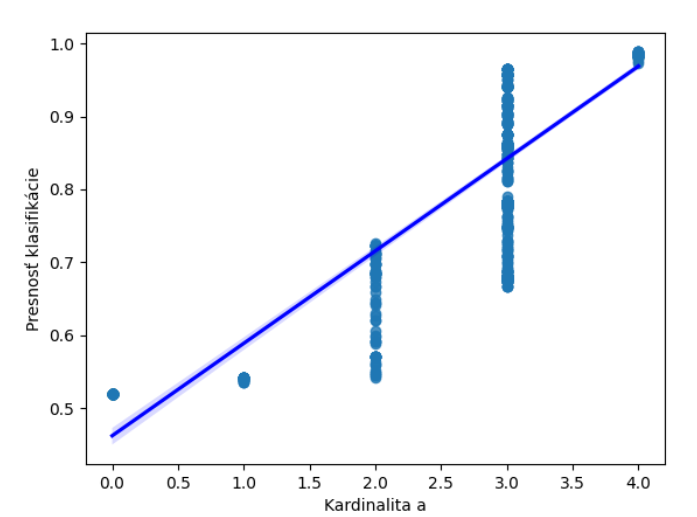
\includegraphics[width=6cm]{kar_acc.png} }}%
    \qquad
    \subfloat[\centering Kardinalita vs Phi($\mu$)]{{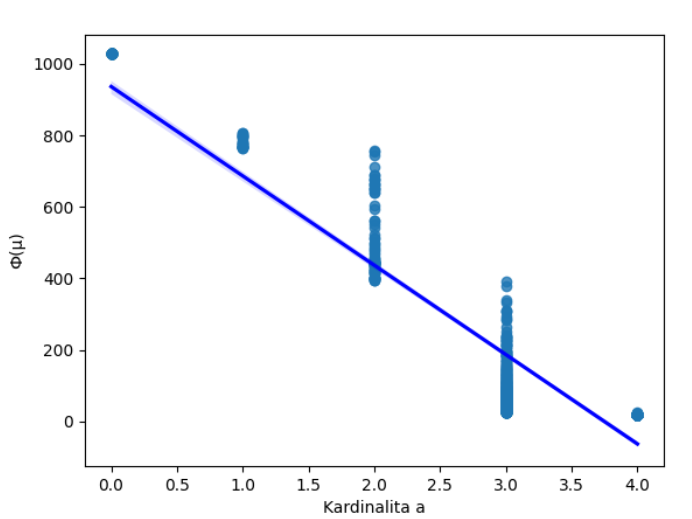
\includegraphics[width=6cm]{kar_phi.png} }}%
    \caption{Vplyv Kardinality na rôzne metriky}%
    \label{fig:kar}%
\end{figure} 
\begin{figure}[b]%
    \centering
    \subfloat[\centering $\mu$ vs Presnosť]{{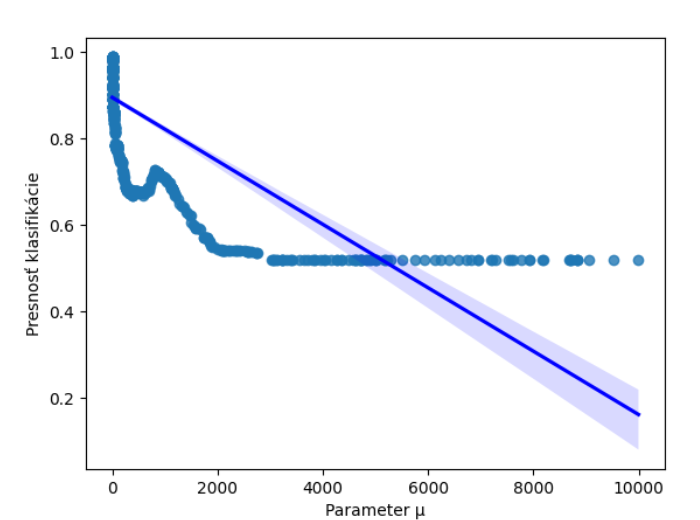
\includegraphics[width=6cm]{mu_acc.png} }}%
    \qquad
    \subfloat[\centering $\mu$ vs $\phi$($\mu$)]{{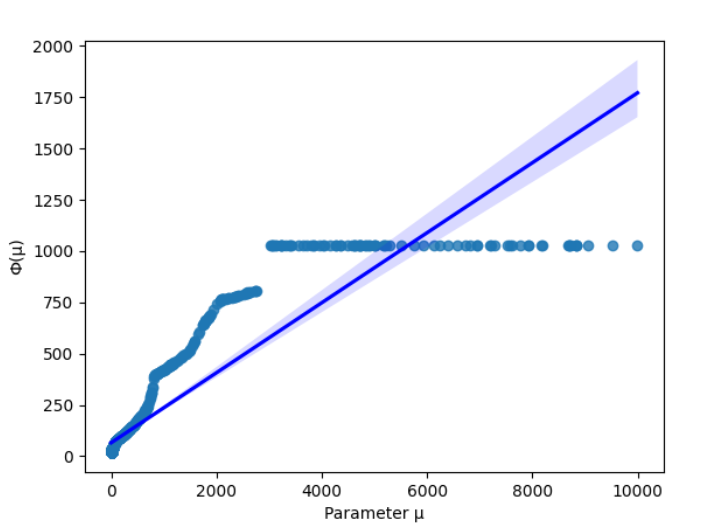
\includegraphics[width=6cm]{mu_phi.png} }}%
    \caption{Vplyv $\mu$ na rôzne metriky}%
    \label{fig:mu}%
\end{figure}
\end{document}

\end{document}
